\chapter{Progress on the Open Problems}\label{ch:progress}\index{product formula}\index{Laguerre P\'olya class}\index{likelihood ratio order}\index{effective coupling}\index{Parisi, G.}\index{string tension}\index{scale factor}

This chapter reports our own progress, made in this book, on the open problems listed in Chapter~\ref{ch:path}. It is not a survey of the literature: the recent work of others on lattice Yang Mills is discussed in Section~\ref{ch:missing}, and the history in Chapter~\ref{ch:programme}. The SU(2) half of the second problem is closed: the likelihood ratio property of the SU(2) heat kernel, on which the monotonicity of the projected ladder rests, is now a theorem at every time, by a product formula for the heat kernel. The chapter also proves the weak coupling expansion of the ladder (Theorems~\ref{thm:expansion} and~\ref{thm:expansionN}), total positivity of convolution (Theorem~\ref{thm:tp2}), and that the ladder contracts (Theorem~\ref{thm:scaledmlr} and Corollary~\ref{cor:contracts}); the rest are quantitative tests of the ladder against lattice data. They give an honest mixed verdict: the ladder predicts the rate of running to within ten or fifteen percent, has about half the correct two loop coefficient, and misplaces the crossover to strong coupling.

\section{A product formula for the heat kernel}

Write the SU(2) heat kernel in the normalisation of Section~\ref{ch:verification},
\[
K_t(\theta)=\sum_{n\ge1}n\,e^{-(n^2-1)t/4}\,\frac{\sin n\theta}{\sin\theta},
\]
and put $c=\cos\theta$ and $C_n(t)=\cosh\big((2n-1)t/4\big)$.

\begin{theorem}[product formula]\label{thm:product}
For every $t>0$,
\[
K_t(\theta)=K_t(\pi/2)\prod_{m\ge1}\Big(1+\frac{\cos\theta}{\gamma_m(t)}\Big),
\]
where $\gamma_1<\gamma_2<\cdots$ are the roots of
\[
\sum_{n\ge1}\frac{1}{C_n(t)-\gamma}=0,\qquad C_m(t)<\gamma_m(t)<C_{m+1}(t).
\]
In particular every $\gamma_m(t)$ exceeds one. Each $\gamma_m$ is strictly increasing in $t$, with
\[
\gamma_m'(t)=\sum_{n\ge1}w_{mn}\,C_n'(t),\qquad w_{mn}=\frac{(C_n-\gamma_m)^{-2}}{\sum_{l}(C_l-\gamma_m)^{-2}} .
\]
\end{theorem}

\begin{proof}
Let $\nu=e^{-t/4}$ and $\vartheta(\theta)=\sum_{n\in\Z}\nu^{n^2}e^{in\theta}$, the heat kernel of the circle. Since $-\partial_\theta\vartheta=2\sum_{n\ge1}n\nu^{n^2}\sin n\theta$ and $\partial_\theta=-\sin\theta\,\partial_c$,
\[
K_t(\theta)=\frac{e^{t/4}}{2}\,\frac{\mathrm d\vartheta}{\mathrm dc}.
\]
The Jacobi triple product gives $\vartheta=\prod_{n\ge1}(1-\nu^{2n})\cdot P(c)$ with
\[
P(c)=\prod_{n\ge1}\big(1+\nu_n^2+2\nu_nc\big),\qquad \nu_n=\nu^{2n-1}.
\]
As a function of $c$, $P$ is entire of order zero, with simple real zeros at $c=-(1+\nu_n^2)/(2\nu_n)=-C_n(t)$. By Laguerre's theorem~\cite{PS14} the derivative of such a function has only real simple zeros, one in each gap between consecutive zeros of $P$, and is again of order zero. Hadamard's factorisation therefore has no exponential factor, and $P'(c)=P'(0)\prod_m(1+c/\gamma_m)$ with $-\gamma_m\in(-C_{m+1},-C_m)$. The equation for the roots is $P'/P=\sum_n(c+C_n)^{-1}=0$ at $c=-\gamma$.

For the motion of the roots, differentiate $\sum_n(C_n(t)-\gamma_m(t))^{-1}=0$ in $t$; the series converges locally uniformly with its derivative, because $C_n$ grows like $e^{nt/2}$. This gives $\sum_n(C_n'-\gamma_m')(C_n-\gamma_m)^{-2}=0$, which is the stated formula. The weights $w_{mn}$ are positive and sum to one, and $C_n'(t)=\frac{2n-1}{4}\sinh((2n-1)t/4)>0$.
\end{proof}

The proof is the classical fact that the critical points of a function with real zeros move as convex combinations of the velocities of the zeros. Here every zero $-C_n(t)$ moves to the left as $t$ grows, so every critical point does too.

\begin{corollary}[likelihood ratio property]\label{cor:mlrall}
For every $t>0$ and $\theta\in(0,\pi)$,
\[
\partial_t\,\partial_\theta\log K_t(\theta)=\sin\theta\sum_{m\ge1}\frac{\gamma_m'(t)}{(\gamma_m(t)+\cos\theta)^2}>0 .
\]
The SU(2) heat kernel has strictly monotone likelihood ratio in time, the hypothesis of Lemma~\ref{lem:mlrB} holds, and the projected Migdal Kadanoff map $R$ is increasing at every coupling and for every scale factor $b$.
\end{corollary}

\begin{corollary}[log concavity]\label{cor:logconc}
For every $t>0$ the heat kernel is strictly log concave as a function of $c=\cos\theta$ on $[-1,1]$, with $\partial_c^2\log K_t=-\sum_m(\gamma_m+c)^{-2}$. The same holds for every power $K_t^k$, hence for every plaquette law produced by bond moving from a heat kernel law.
\end{corollary}

\begin{corollary}[Thorin form]\label{cor:thorinform}
For every $t>0$, with $x=\cos\theta$,
\[
\frac{K_t(\pi/2)}{K_t(\theta)}=\prod_{m\ge1}\frac{\gamma_m(t)}{\gamma_m(t)+x}=\E\,e^{-xT_t},\qquad T_t=\sum_{m\ge1}\frac{E_m}{\gamma_m(t)},
\]
with independent standard exponential $E_m$. So the reciprocal of the heat kernel, as a function of $x=\cos\theta$, is the Laplace transform of a generalized gamma convolution whose Thorin measure $\sum_m\delta_{\gamma_m(t)}$ has integer masses and is supported on $(1,\infty)$, beyond the edge of the group, with atoms moving to the right as $t$ grows.
\end{corollary}
\begin{proof}
By Theorem~\ref{thm:product}, $K_t=K_t(\pi/2)\prod_m(1+x/\gamma_m(t))$ with every $\gamma_m(t)>1$, increasing in $t$, and $\sum_m1/\gamma_m(t)<\infty$ because $\gamma_m(t)>C_m(t)$; so $K_t$ is in the class $\mathcal L$ of Chapter~\ref{ch:zeros}, and $\E\,e^{-xE_m/\gamma_m}=\gamma_m/(\gamma_m+x)$ for $x>-\gamma_m$.
\end{proof}

Three remarks. First, as a function of $c$ the heat kernel belongs to the Laguerre P\'olya class~\cite{PS14}: it is a limit of polynomials with only real zeros, all outside the interval $[-1,1]$ on which it is a density. This is the P\'olya class~\cite{Po26}, in which the Riemann $\Xi$ function~\cite{Ri59} lies exactly when the Riemann Hypothesis holds, and the argument above is of de Bruijn Newman type~\cite{dB50,Ne76}: under the heat flow the zeros move monotonically, here away from the support. Section~\ref{ch:rhbooks} (Chapter~\ref{ch:kacyang}) returns to this. Second, the product formula gives a sampler: $K_t$ is a product of linear factors in $c$, so it can be bounded above by its first factors for rejection sampling at any $t$. Third, the corollaries are strict for every $t>0$ and every $\theta\in(0,\pi)$.

\begin{figure}[t]
\centering
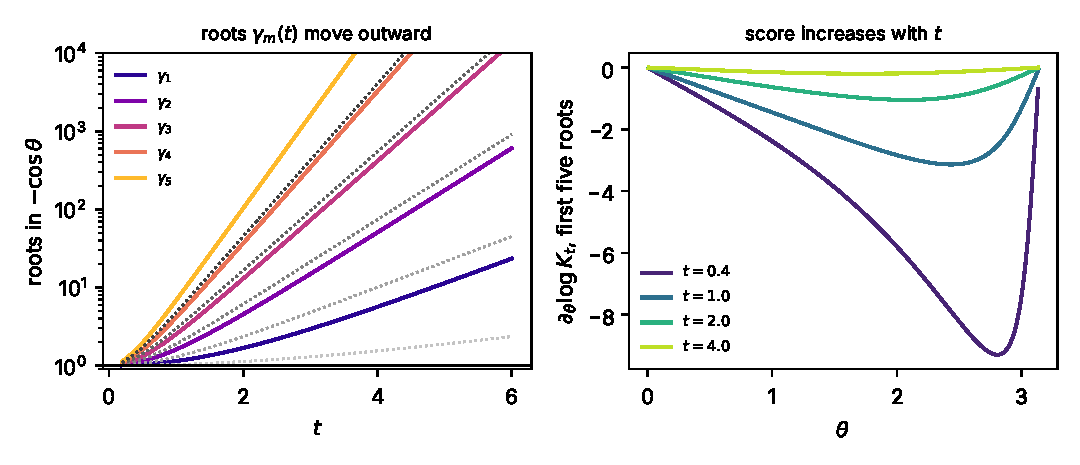
\includegraphics[width=\textwidth]{figures/heat_roots.pdf}
\caption[Roots of the SU(2) heat kernel]{Left: the first five roots $\gamma_m(t)$ of the heat kernel in the variable $-\cos\theta$, solid, interlaced with the zeros $C_n(t)=\cosh((2n-1)t/4)$ of the theta function, dotted. All move outward as $t$ grows. Right: the score $\partial_\theta\log K_t$ computed from the first five roots; it increases with $t$ at every angle.}
\label{fig:heatroots}
\end{figure}

We checked the product formula numerically: with forty roots, computed in forty digit arithmetic, the ratio of the character series to the product is constant in $\theta$ to $10^{-8}$ at $t=1$, $10^{-17}$ at $t=2$ and $10^{-31}$ at $t=4$, and every computed root increases with $t$ (Figure~\ref{fig:heatroots}). Figure~\ref{fig:mlrratios} shows the property directly, and Figure~\ref{fig:mlrheat} maps the mixed partial over the whole time range, computed independently from the Poisson resummed image sum; its normalised minimum on $[0.04,3.41]$ is $0.67$.

\begin{figure}[t]
\centering
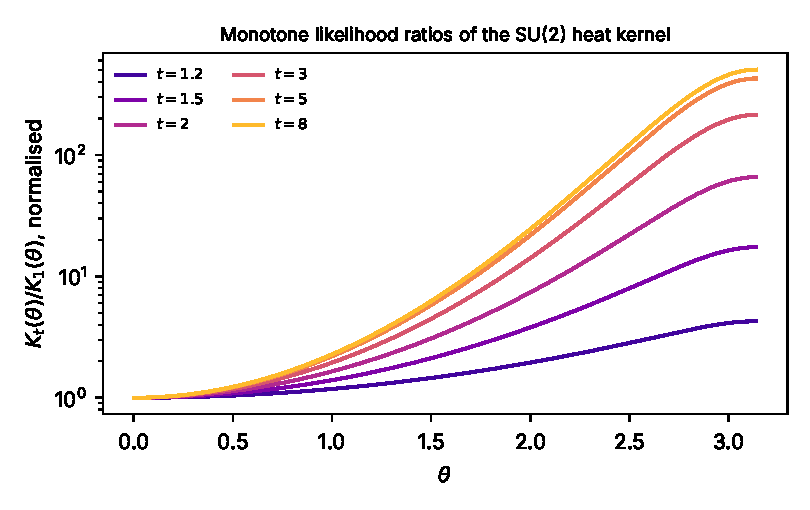
\includegraphics[width=0.85\textwidth]{figures/mlr_ratios.pdf}
\caption[Likelihood ratios of the SU(2) heat kernel]{Likelihood ratios $K_t(\theta)/K_1(\theta)$ of the SU(2) heat kernel, normalised at $\theta=0$, for six times. Each is increasing in $\theta$, which is the monotone likelihood ratio property.}
\label{fig:mlrratios}
\end{figure}

\begin{figure}[t]
\centering
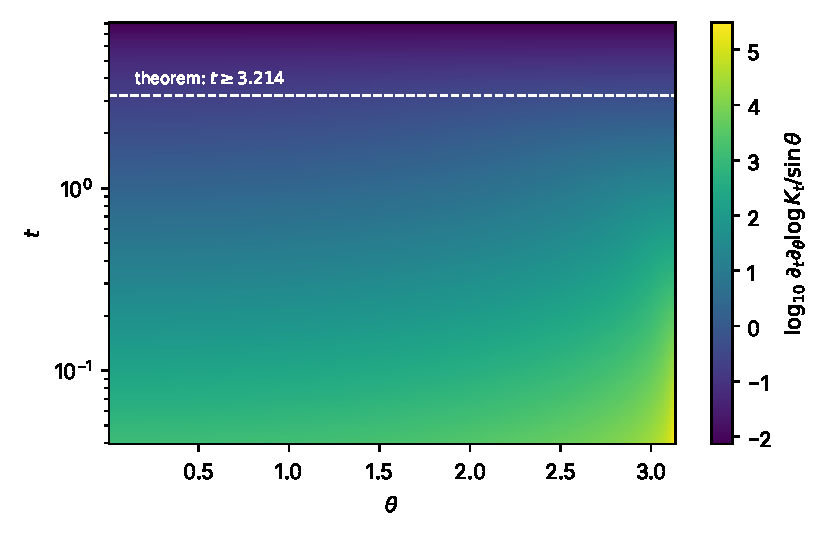
\includegraphics[width=0.9\textwidth]{figures/mlr_heatmap.pdf}
\caption[The mixed partial of the log heat kernel]{The normalised mixed partial $\partial_t\partial_\theta\log K_t(\theta)/\sin\theta$ on a logarithmic colour scale, computed from the image sum. It is positive everywhere, as Corollary~\ref{cor:mlrall} requires. The dashed line marks $t=3.214$, above which the elementary bound of Proposition~\ref{thm:mlrlarge} also applies.}
\label{fig:mlrheat}
\end{figure}

\section{Two other proofs, and the Wilson law}

Before finding the product formula we had two partial arguments. Both are worth recording because they generalise in different directions.

\begin{proposition}[elementary bound at large time]\label{thm:mlrlarge}
With $\varepsilon_n(t)=n\,e^{-(n^2-1)t/4}$, let
\begin{align*}
\Phi(t)={}&6\varepsilon_2-\sum_{n\ge3}\frac{(n^2-1)(n^3-n)}{3}\,\varepsilon_n\\
&-\frac{\big(\sum_{n\ge2}(n^2-1)n\,\varepsilon_n\big)\big(\sum_{m\ge2}\frac{m^3-m}{3}\varepsilon_m\big)}{1-\sum_{n\ge2}n\,\varepsilon_n}.
\end{align*}
Then $4\,\partial_t\partial_\theta\log K_t(\theta)\ge \Phi(t)\sin\theta/K_t(\theta)$ whenever the denominator is positive, and $\Phi(t)>0$ for all $t\ge3.2140$.
\end{proposition}

\begin{proof}
Differentiate the character series term by term and use three bounds: $\partial_\theta U_1(\cos\theta)=-2\sin\theta$ for the leading term; the bound $|U_{n-1}'|\le U_{n-1}'(1)=(n^3-n)/3$ on $[-1,1]$ for the rest, which holds because $U_{n-1}'=2C^{(2)}_{n-2}$ is a Gegenbauer polynomial of positive index and so attains its largest modulus on $[-1,1]$ at $x=1$; and $|U_{n-1}|\le n$. The function $e^{3t/4}\Phi(t)$ is increasing with limit $12$, and a bisection in thirty digit arithmetic locates its zero at $3.2140$.
\end{proof}

The proof above uses the Chebyshev series of SU(2), so the proposition is stated for SU(2) only. The argument uses little beyond the gap of the Laplacian between its first two levels, so we expect it to extend to any compact group and to SU(3), where no product formula in one variable is available; we have not written the extension.

The second argument is a maximum principle. Let $\rho_t$ solve the radial heat equation $\partial_t\rho=\frac14(\rho''+2\cot\theta\,\rho')$ on $(0,\pi)$, and put $v=\partial_\theta\log\rho$ and $z=\partial_tv$. Then
\[
4\,\partial_tz=z''+(2v+2\cot\theta)\,z'+\Big(2v'-\frac{2}{\sin^2\theta}\Big)z ,
\]
a linear parabolic equation with $z=0$ at both ends by symmetry. If $z\ge0$ at one time it stays nonnegative, by the maximum principle (Section~\ref{ch:proofs2} of the appendix). For the heat kernel this reduces the property at all times to the property at arbitrarily small times. For other initial laws it gives new information.

\begin{proposition}[Wilson law]\label{prop:wilsonflow}
Let $\rho_0(\theta)\propto e^{\kappa\cos\theta}$ be the Wilson~\cite{Wi74} plaquette law and $\rho_t$ its heat flow. At $t=0$,
\[
4\,\partial_t\partial_\theta\log\rho_t=\kappa\sin\theta\,(3+2\kappa\cos\theta).
\]
Hence the family $(\rho_t)_{t\ge0}$ has monotone likelihood ratio in time if and only if $\kappa\le3/2$.
\end{proposition}

\begin{proof}
With $v=-\kappa\sin\theta$, compute $v''+2vv'+2\cot\theta\,v'-2v/\sin^2\theta=\kappa\sin\theta+2\kappa^2\sin\theta\cos\theta+2\kappa\sin\theta$. This is nonnegative on $(0,\pi)$ exactly when $\kappa\le3/2$, and the maximum principle propagates the sign. For $\kappa>3/2$ the property fails near $\theta=\pi$ at small times.
\end{proof}

A numerical check agrees: the minimum of the mixed partial over a grid of times and angles is positive for $\kappa=0.5$, $1$ and $1.5$ and negative for $\kappa=2$ and $3$. The threshold has a meaning. The Wilson law at $\kappa>3/2$ has too little mass near the antipode $-1$ relative to any heat kernel, and the flow first repairs that. This is a precise version of the statement that the Wilson action and the heat kernel action differ near the centre element, the region responsible for the lattice artefacts that the positive plaquette and heat kernel actions were designed to remove.

\section{A first look at SU(3)}

For SU(3) the heat kernel is a function on the maximal torus, of two angles, and there is no product formula in one variable. The natural analogue of the likelihood ratio property is along rays from the identity: for $\theta=r\mathbf e$ with $\mathbf e$ a direction in the Weyl alcove, is $\partial_t\partial_r\log K_t(r\mathbf e)\ge0$? We computed the heat kernel from its character expansion with all representations of Dynkin labels $p+q\le60$, on four rays and seventy times in $[0.12,6]$, out to $98$ percent of the distance at which the ray leaves the alcove (Figure~\ref{fig:su3mlr}).

\begin{figure}[t]
\centering
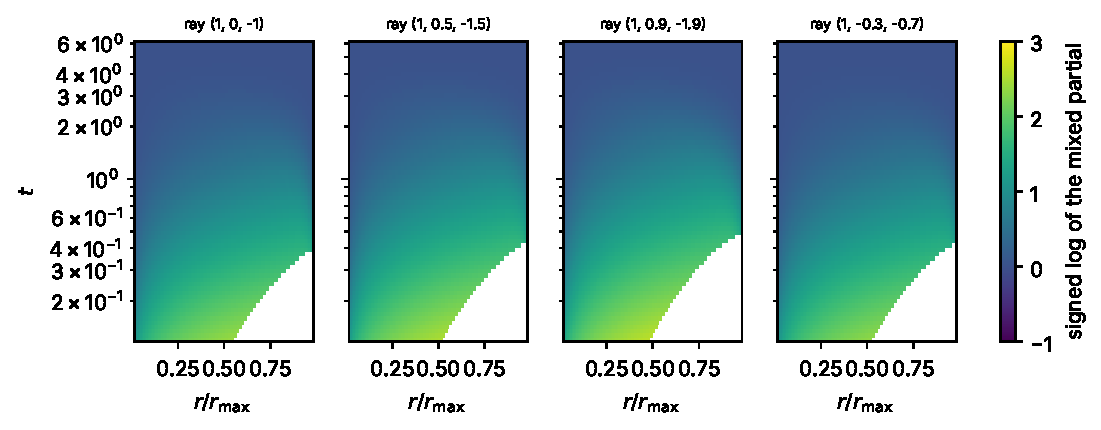
\includegraphics[width=\textwidth]{figures/su3_mlr.pdf}
\caption[The likelihood ratio property for SU(3) along rays]{The mixed partial $\partial_t\partial_r\log K_t(r\mathbf e)$ of the SU(3) heat kernel along four rays from the identity in the Weyl alcove, on a signed logarithmic colour scale. It is positive wherever the kernel exceeds $10^{-6}$; the blank corner at small time and large distance is where the character sum loses precision.}
\label{fig:su3mlr}
\end{figure}

On every ray the mixed partial is positive at every grid point where the kernel is larger than $10^{-6}$, about ninety percent of the grid; the excluded points lie at small time and large distance, where the kernel is smaller than the rounding error of the sum. The minimum over the grid is about $3\times10^{-4}$; at large time and small distance the mixed partial tends to zero, as it does for SU(2). So the property holds numerically for SU(3) along rays. A proof might come from the Gaussian sum over the coroot lattice, in which each image is log supermodular in $(t,r)$ and the Weyl denominator does not depend on $t$, or from a two variable form of the Laguerre argument.

\begin{quote}
\textsc{Status.} The likelihood ratio property of the SU(2) heat kernel is a theorem at every time. The projected ladder map is therefore monotone without numerical input, the contraction $R(\beta)<\beta$ is proved outright in Corollary~\ref{cor:contracts}, and the covering of Remark~\ref{prop:coverB} needs only interval arithmetic for the map itself to become a computer assisted proof. For SU(3) numerics give the property along rays; a proof, at large time or otherwise, is open.
\end{quote}

\section{A first test against lattice data}

The ladder predicts that the lattice spacing halves each time $\beta$ increases by the decrement, $1/4$ at weak coupling for SU(2) with $b=2$. Hence $d\log a/d\beta=-4\log2=-2.77$. Perturbation theory predicts the asymptotic value $-1/(4Nb_0)=-2.69$ at one loop and, with the two loop correction at $\beta=2.5$, a local slope of $-2.52$. We compare with the string tension of the Wilson action measured on large lattices, $a\sqrt\sigma=0.4690$, $0.3690$, $0.2660$, $0.1871$ and $0.1207$ at $\beta=2.2$, $2.3$, $2.4$, $2.5$ and $2.635$, as collected in Teper's review~\cite{Te98}.

\begin{figure}[t]
\centering
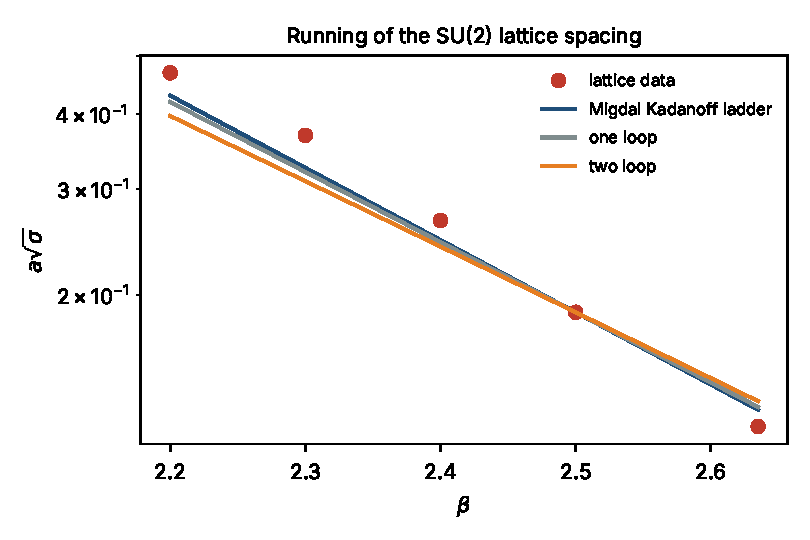
\includegraphics[width=0.85\textwidth]{figures/scaling_test.pdf}
\caption[The Migdal Kadanoff ladder against SU(2) lattice data]{The string tension $a\sqrt\sigma$ of SU(2) with the Wilson action, against the running predicted by the Migdal Kadanoff ladder and by one and two loop perturbation theory, all normalised at $\beta=2.5$.}
\label{fig:scaling}
\end{figure}

The data have a fitted slope of $-3.18$, with local slopes $-2.40$, $-3.27$, $-3.52$ and $-3.25$ between successive couplings (Figure~\ref{fig:scaling}). In this window the lattice spacing therefore shrinks about fifteen percent faster than the ladder predicts, and about twenty five percent faster than two loop perturbation theory. This is the well known failure of asymptotic scaling for the Wilson action at intermediate coupling, which is usually cured by replacing the bare coupling with an effective coupling defined from the measured plaquette, as Parisi proposed~\cite{Pa80}. In its weak coupling limit, $-2.77$, the ladder slope falls between one loop and the data. Its strong coupling corrections, visible in the decrements of Section~\ref{ch:verification}, $0.2623$ at $\beta=2$ rather than $0.25$, slow the running and so push the other way: integrated from the computed decrements the ladder slope is $-2.67$, slightly shallower than one loop and further from the data.

Two conclusions follow. The caricature is not quantitatively accurate at $\beta\approx2.5$, and any comparison theorem for step 4 must allow a bracket of at least this width. And the natural fix is the same as in lattice practice: run the ladder in an effective coupling. Because the ladder carries the whole plaquette law rather than a single number, its own $u_2$, the mean plaquette, supplies such a coupling without further input. The next two sections carry out that test.


\section{The ladder in an effective coupling}

Parisi's effective coupling~\cite{Pa80} replaces the bare $\beta$ by the value $\beta_E$ at which the leading weak coupling formula reproduces the measured plaquette. For SU(2) that formula is $\langle\tfrac12\operatorname{tr}U_p\rangle=1-3/(4\beta)$, so
\[
\beta_E=\frac{3}{4\,(1-\langle\tfrac12\operatorname{tr}U_p\rangle)} .
\]
We measured the plaquette ourselves, with a vectorised checkerboard heat bath of Kennedy and Pendleton type~\cite{KP85} on an $8^4$ lattice, sixty sweeps of equilibration and six hundred of measurement at each coupling. The plaquettes are $0.56997$, $0.60305$, $0.62976$, $0.65264$ and $0.67629$ at $\beta=2.2$, $2.3$, $2.4$, $2.5$ and $2.635$, with standard errors between $1\times10^{-4}$ and $4\times10^{-4}$. The effective couplings are $\beta_E=1.744$, $1.889$, $2.026$, $2.159$ and $2.317$.

\begin{figure}[t]
\centering
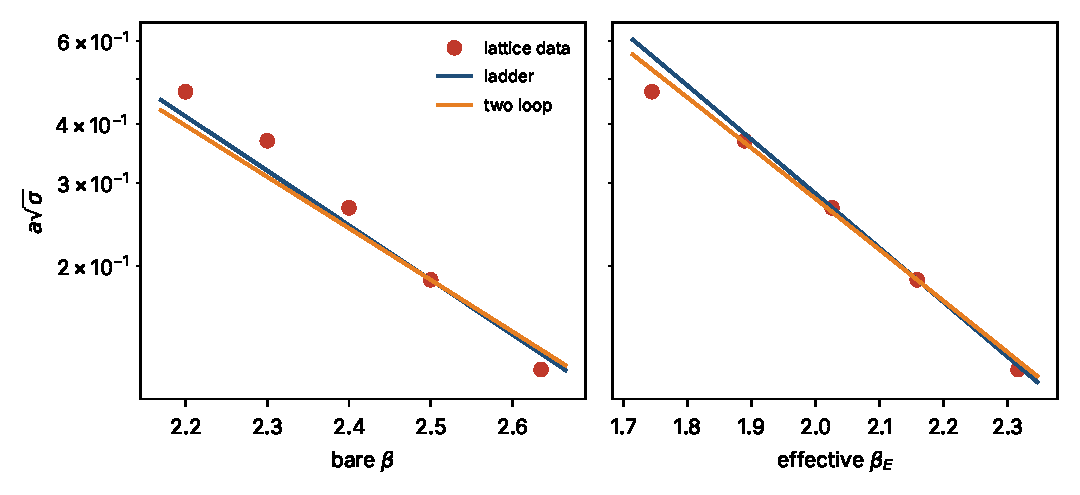
\includegraphics[width=\textwidth]{figures/effective_coupling.pdf}
\caption[The ladder in bare and effective coupling]{SU(2) string tension data against the Migdal Kadanoff ladder and two loop perturbation theory, as functions of the bare coupling (left) and of Parisi's effective coupling (right). The ladder is integrated from the computed decrements $\beta-R(\beta)$, not from their weak coupling limit.}
\label{fig:effcoupling}
\end{figure}

Figure~\ref{fig:plaq4d} places our plaquettes against the strong and weak coupling expansions and the exact two dimensional law.

\begin{figure}[t]
\centering
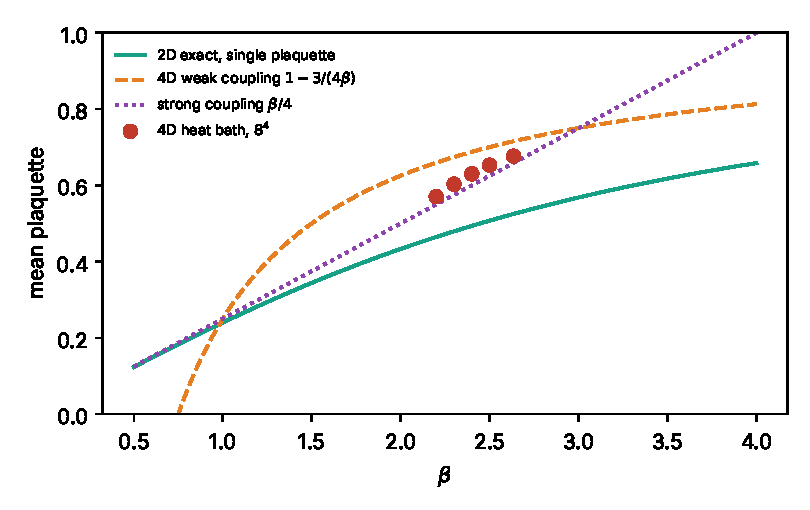
\includegraphics[width=0.85\textwidth]{figures/plaquette_4d.pdf}
\caption[Four dimensional SU(2) plaquette]{Mean plaquette of four dimensional SU(2) from our $8^4$ heat bath runs, against the strong coupling expansion $\beta/4$, the weak coupling formula $1-3/(4\beta)$ that defines $\beta_E$, and the exact single plaquette law of two dimensions.}
\label{fig:plaq4d}
\end{figure}

In the effective coupling the picture changes (Figure~\ref{fig:effcoupling}). The data have slope $-2.40$; two loop perturbation theory gives $-2.48$, within four percent, and the ladder, integrated from its computed decrements $0.268$, $0.265$, $0.263$ and $0.262$ at $\beta=1.5$, $1.7$, $1.9$ and $2.1$, gives $-2.64$, about ten percent too steep. The residual scatter about each prediction is $0.047$ for two loops and $0.066$ for the ladder, against $0.104$ and $0.082$ in the bare coupling. So the effective coupling cures most of the failure of scaling for both, as it does in lattice practice, and the ladder flips from running too slowly, by fifteen percent in the weak coupling slope or nineteen percent in the computed decrements, to ten percent too fast.

\section{The ladder's two loop coefficient}

The remaining discrepancy has a clean source. Write the decrement per doubling of the lattice spacing as $\delta(\beta)=d\beta/d\log_2(1/a)$. Two loop perturbation theory gives
\[
\delta_{\mathrm{pert}}(\beta)=\log2\,\Big(4Nb_0+\frac{8N^2b_1}{\beta}\Big)+O(\beta^{-2})=0.2575+\frac{0.0403}{\beta}+O(\beta^{-2})
\]
for SU(2), with $b_0=11N/(48\pi^2)$ and $b_1=34N^2/(3(16\pi^2)^2)$. The coefficient of $1/\beta$ is unchanged by any shift $\beta\mapsto\beta+c$, which is how a change of scheme acts at this order, so it can be compared across schemes. The ladder at $b=2$ has $\delta_{\mathrm{MK}}(\beta)=0.2500+0.021/\beta$ above $\beta=20$ (Section~\ref{ch:verification}). Figure~\ref{fig:decpert} compares the two decrement curves over the whole range of couplings. The ladder therefore reproduces the one loop coefficient to three percent and the two loop coefficient to about fifty two percent. Its approach to strong coupling is too abrupt: it does not slow down enough as the coupling grows.


\begin{figure}[t]
\centering
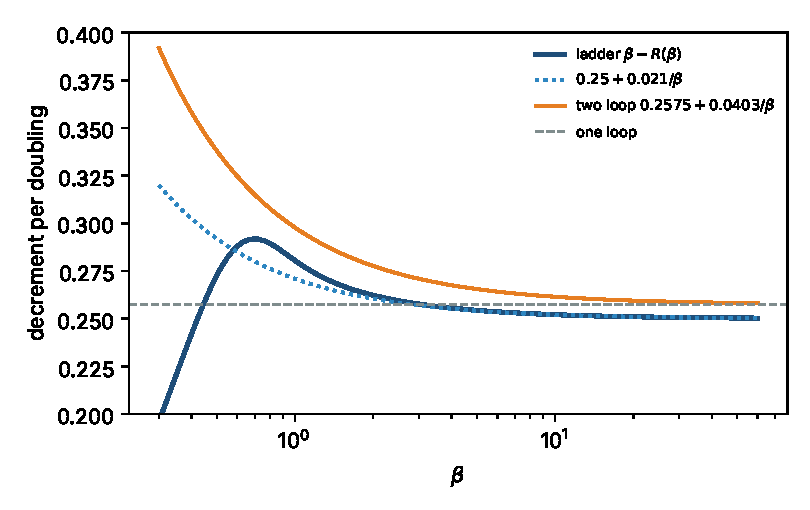
\includegraphics[width=0.85\textwidth]{figures/decrement_vs_pert.pdf}
\caption[Ladder decrement against perturbation theory]{The computed ladder decrement $\beta-R(\beta)$ at $b=2$, its fit $0.25+0.021/\beta$, and the two loop perturbative decrement $0.2575+0.0403/\beta$. The ladder tends to $0.25$, three percent below one loop, with about half the two loop coefficient of $1/\beta$, and peaks near $\beta=0.7$ before falling at strong coupling.}
\label{fig:decpert}
\end{figure}

\begin{quote}
\textsc{Status.} In Parisi's effective coupling the ladder predicts the running of the SU(2) string tension over $2.2\le\beta\le2.635$ to within ten percent; two loop perturbation theory does better, to four percent. The ladder's own two loop coefficient is $0.021$ against the true $0.0403$. Any comparison theorem for step 4 must therefore allow a bracket that corrects the second order running, and an improved ladder, for example with $b$ varied along the flow or with the bond moving step weighted by the measured plaquette, should first be tested on this coefficient.
\end{quote}

\section{Can the scale factor repair the ladder?}

The ladder has one free parameter, the scale factor $b$, which need not be an integer: bond moving raises the plaquette law to the power $b^2$ and decimation raises character coefficients to the power $b^2$, and both make sense for real $b>1$. Per doubling of the lattice spacing the decrement is $a(b)+c(b)/\beta$ with
\[
a(b)=\frac{1-b^{-2}}{3\log_2b},
\]
from Remark~\ref{prop:decrementB}. We computed $c(b)$ by fitting the decrement on $20\le\beta\le150$; the fitted $a(b)$ agrees with the formula to five digits.

\begin{center}
\small
\begin{tabular}{cccccccccc}
\toprule
$b$ & 1.2 & 1.4 & 1.6 & 1.8 & 1.925 & 2 & 2.2 & 3 \\ \midrule
$a(b)$ & 0.387 & 0.336 & 0.300 & 0.272 & 0.2576 & 0.250 & 0.232 & 0.187 \\
$c(b)$ & 0.090 & 0.057 & 0.039 & 0.028 & 0.0232 & 0.0208 & 0.016 & 0.007 \\
\bottomrule
\end{tabular}
\end{center}

\begin{figure}[t]
\centering
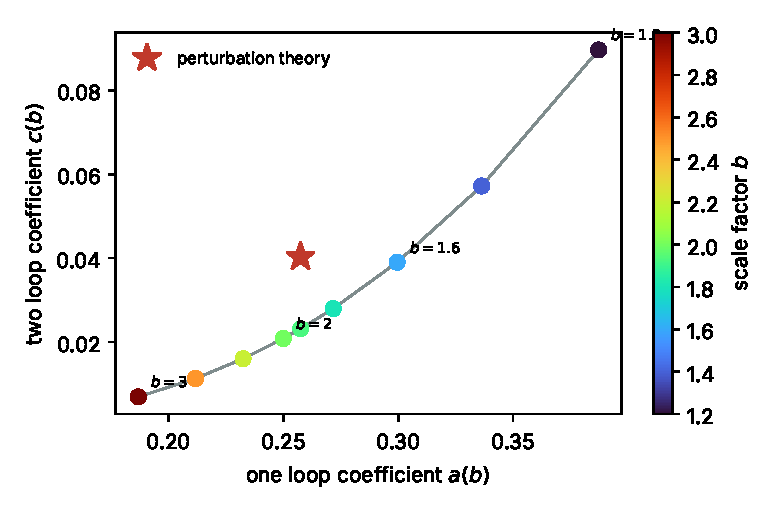
\includegraphics[width=0.8\textwidth]{figures/ladder_b.pdf}
\caption[One and two loop coefficients of the ladder as the scale factor varies]{The one loop and two loop coefficients $(a(b),c(b))$ of the ladder as the scale factor $b$ varies, coloured by $b$, and the perturbative values $(0.2575,0.0403)$, marked by a star. The curve passes below the star: no scale factor matches both.}
\label{fig:ladderb}
\end{figure}

At $b=2$ the two loop coefficient is $0.02083$, which is $1/48$ to the accuracy of the fit; the next section proves it. The scale factor $b_*=1.925$ reproduces the one loop coefficient $0.2575$ exactly, and there $c=0.0232$, still fifty eight percent of the true $0.0403$. Matching the coefficient $c$ itself instead needs $b=1.58$, where the one loop coefficient is seventeen percent too large. Figure~\ref{fig:ladderb} shows the curve $(a(b),c(b))$ passing below the perturbative point. The scale factor alone cannot repair the ladder; the second order error is structural, a property of bond moving, and an improved ladder must change the bond moving step itself.

\section{The weak coupling expansion of the ladder, exactly}

The numerical value $c(2)=0.02083$ of the last section suggested $1/48$. The whole expansion can in fact be computed in closed form, and the scale factor enters through one rational function.

\begin{theorem}[weak coupling expansion]\label{thm:expansion}
Let bond moving have power $k$ and decimation power $D$, and let $t=2/\beta$ be the heat kernel time. For SU(2) the projected ladder map is, as $t\to0$,
\[
t'=\frac{D}{k}\,t\,\Big[1+\Big(1-\frac1k\Big)\Big(\frac t6+\frac{t^2}{36}\Big)+\frac{(k-1)(2k^2+2k-3)}{432\,k^3}\,t^3+O(t^4)\Big].
\]
In four dimensions, $k=D=b^2$, the decrement is
\[
\beta-R(\beta)=\frac{b^2-1}{3b^2}+\frac{b^2-1}{9b^4}\,\frac1\beta+\frac{(b^2-1)(2b^2-1)}{54\,b^6}\,\frac1{\beta^2}+O(\beta^{-3}),
\]
which for $b=2$ is $\frac14+\frac{1}{48\beta}+\frac{7}{1152\beta^2}$.
\end{theorem}

\begin{proof}
For small $t$ the heat kernel is its leading image up to terms of relative size $e^{-4\pi^2/t}$ away from the antipode, and the antipode carries exponentially small mass: $K_t(\theta)\propto(\theta/\sin\theta)\,e^{-\theta^2/t}$. After bond moving the law of the angle has density proportional to
\[
K_t(\theta)^k\sin^2\theta\ \propto\ \theta^2\Big(\frac{\theta}{\sin\theta}\Big)^{k-2}e^{-\theta^2/\tau},\qquad\tau=\frac tk .
\]
This is the radial law of a Gaussian vector in $\R^3$ with a weight $w=\exp\big((k-2)\log(\theta/\sin\theta)\big)$, and $\log(\theta/\sin\theta)=\theta^2/6+\theta^4/180+\theta^6/2835+\cdots$. The new coefficient is $u_2=\E[w\cos\theta]/\E[w]$, where both expectations are polynomials in $\tau$ at each order because the moments of $\theta^2e^{-\theta^2/\tau}$ are $\E\theta^{2j}=\tau^j\,\Gamma(j+\frac32)/\Gamma(\frac32)$. Decimation gives $t'=-\frac43D\log u_2$. Expanding to the stated order is a finite computation, done in exact rational arithmetic by the script of Appendix~\ref{ch:code}.
\end{proof}

The case $k=2$ can be done by hand and checks the series. The weight is then one, the law is exactly the radial Gaussian, and $\E\cos|X|=(1-\sigma^2)e^{-\sigma^2/2}$ with $\sigma^2=t/4$, so $t'=D\big[\frac t6-\frac43\log(1-\frac t4)\big]=D\big[\frac t2+\frac{t^2}{24}+\frac{t^3}{144}+\cdots\big]$, in agreement with the theorem. The theorem also agrees with the numerical decrements of Section~\ref{ch:verification}: at $b=2$ it gives $0.25441$ at $\beta=5$ and $0.2521$ at $\beta=10$, against the computed $0.2544$ and $0.2521$.

Three consequences.

First, the leading term is Remark~\ref{prop:decrementB}, with $\E S_{\mathrm{BPY}}=\frac13$ appearing as twice the coefficient $\frac16$ of $\theta^2$ in $\log(\theta/\sin\theta)$. The higher coefficients $\frac1{180}$ and $\frac1{2835}$, multiplied by $2^jj!$ for the coefficient of $\theta^{2j}$, are, up to such factors, the higher cumulants of the Biane, Pitman and Yor variable~\cite{BPY}. The expansion of the ladder is the cumulant expansion of $S_{\mathrm{BPY}}$.

Second, the comparison with perturbation theory can be made in a form that does not depend on the scheme. Write one step as $t'=t+At^2+A't^3$. For a flow $\mathrm dt/\mathrm d\log a=\alpha t^2(1+\rho t)$ integrated over a scale factor, $(A'-A^2)/A=\rho$, and $\rho$ is invariant under $t\mapsto t+ct^2$. The true theory has $\rho=2b_1/b_0=17N/(44\pi^2)$, which is $0.0783$ for SU(2). The ladder has
\[
\rho_{\mathrm{ladder}}=\frac{A'-A^2}{A}=\frac{1}{6b^2},
\]
which is $0.0417$ at $b=2$, fifty three percent of the truth. The two values of $\rho$ agree at $b=1.459$, where the one loop coefficient is twenty six percent too large; at $b=1.925$, where one loop is exact, $\rho_{\mathrm{ladder}}=0.0450$. The curve of Figure~\ref{fig:ladderb} is now explicit, and the statement that no scale factor matches both coefficients is a theorem: one needs $(1-b^{-2})/(3\log_2b)=0.2575$ and $1/(6b^2)=0.0783$ at once.

Third, the infinitesimal ladder exists. As $b\to1$ the step becomes the flow $\mathrm dt/\mathrm d\log b=\frac{t^2}{3}\big(1+\frac t6+\cdots\big)$, whose one loop coefficient is $1.79$ times the true one. The Migdal Kadanoff approximation is not improved by making the steps small; its accuracy at $b=2$ is an accident of that scale factor; for the approximation itself see~\cite{Mi75,Ka76}.

In $d$ dimensions the same theorem, with $k=b^{d-2}$ and $D=b^2$, gives $t'=b^{4-d}t\,[1+(1-b^{2-d})(t/6+t^2/36)+\cdots]$. In three dimensions the time grows by the factor $b$ at every step and the curvature terms are corrections; in two they vanish identically and the map is exact.

\section{The expansion for SU(N)}

The same computation can be done on the maximal torus of SU(N). At small time the heat kernel is $\prod_{i<j}J(\phi_i-\phi_j)\,e^{-|\phi|^2/(2t)}$ with $J(x)=(x/2)/\sin(x/2)$, the Haar density is $\prod_{i<j}\sin^2((\phi_i-\phi_j)/2)$, and after bond moving the law on the torus is a Gaussian on the Lie algebra, in radial form, with the weight $\prod_{i<j}J(\phi_i-\phi_j)^{k-2}$. Normalise the time by $u_F=e^{-C_Ft}$ for the fundamental character, with $C_F=(N^2-1)/(2N)$, so that $\beta=2N/g^2=N/t$.

\begin{theorem}\label{thm:expansionN}
For every $N\ge2$ the projected ladder map is
\[
t'=\frac Dk\,t\,\Big[1+\Big(1-\frac1k\Big)\Big(\frac{Nt}{12}+\Big(\frac{Nt}{12}\Big)^2\Big)+O(t^3)\Big],
\]
so that in four dimensions, with $k=D=b^2$,
\[
\beta-R(\beta)=\frac{N^2}{12}\Big(1-\frac1{b^2}\Big)+\frac{N^4}{144\,b^2}\Big(1-\frac1{b^2}\Big)\frac1\beta+O(\beta^{-2}),
\]
and the two loop ratio of the ladder is $\rho_{\mathrm{ladder}}=N/(12b^2)$.
\end{theorem}

\begin{proof}
Let $X$ be the element of the Lie algebra with eigenvalues $i\phi_j$, so that the torus law is the radial part of a law on $\mathfrak{su}(N)$, of dimension $n=N^2-1$, and write $p_r=\sum_j\phi_j^r$, with $p_1=0$. Put $\tau=t/k$ and $m=k-2$. Since $\log J(x)=x^2/24+x^4/2880+\cdots$ and $\sum_{i\ne j}(\phi_i-\phi_j)^2=2Np_2$, $\sum_{i\ne j}(\phi_i-\phi_j)^4=2Np_4+6p_2^2$, the weight is $\exp\big(m(L_2+L_4+\cdots)\big)$ with
\[
L_2=\frac{N}{24}\,p_2,\qquad L_4=\frac{2Np_4+6p_2^2}{5760}.
\]
The factor $e^{mL_2}$ is Gaussian: it changes the variance from $\tau$ to $\tau_{\mathrm e}=\tau/(1-mN\tau/12)$. Let $g(\tau)=\log\E_\tau[\chi_F/N]$ under the Gaussian law of variance $\tau$ on the Lie algebra, and write $g(\tau)=-C_F\tau(1+\mu_1\tau+\mu_2\tau^2+\cdots)$. To first order in $L_4$, which is all that contributes at order $\tau^3$,
\[
\log u_F=g(\tau_{\mathrm e})+m\operatorname{Cov}_\tau\Big(L_4,-\frac{p_2}{2N}\Big)+O(\tau^4).
\]
Under the Gaussian law $p_2/\tau$ is chi squared with $n$ degrees of freedom, so $\operatorname{Cov}(p_2^2,p_2)=4n(n+2)\tau^3$. The direction of $X$ is independent of its length, so $\operatorname{Cov}(p_4,p_2)=4\tau\,\E p_4$, and for traceless Hermitian Gaussian matrices $\E p_4=\tau^2(N^2-1)(2N^2-3)/N$, from the fourth moment $(2N^3+N)\tau^2$ of the Gaussian unitary ensemble after removing the trace. Hence
\begin{align*}
m\operatorname{Cov}\Big(L_4,-\frac{p_2}{2N}\Big)&=-\frac{m\,n\,\tau^3}{2N\cdot5760}\,\big[8(2N^2-3)+24(N^2+1)\big]\\
&=-C_F\,\frac{mN^2\tau^3}{144}.
\end{align*}
The coefficients $\mu_1,\mu_2$ are fixed by the case $k=1$, where the law is the heat kernel itself and $\log u_F=-C_F\tau$ exactly: with $m=-1$ this forces $\mu_1=N/12$ and $\mu_2=N^2/72$. Substituting, with $s=N\tau/12$,
\begin{align*}
\log u_F&=-C_F\tau\,\big[1+(m+1)s+(m+1)(m+2)s^2\big]+O(\tau^4)\\
&=-C_F\tau\,\big[1+(k-1)s+k(k-1)s^2\big]+O(\tau^4),
\end{align*}
and $t'=-D\log u_F/C_F$ is the stated map.
\end{proof}

The values $\mu_1=N/12$ and $\mu_2=N^2/72$ can be checked for $N=2$, where $g(\tau)=-\frac\tau4+\log(1-\frac\tau2)$. The whole theorem was first found, and is confirmed for $N=2$, $3$ and $4$, by exact integration against the squared Vandermonde weight on the torus, with the script in Appendix~\ref{ch:code}; for $N=3$ and $b=2$ the leading term is the decrement $9/16$ of the full numerical flow.

The dependence on $N$ is the notable point. The true two loop ratio is $2b_1/b_0=17N/(44\pi^2)$, also linear in $N$. Hence
\[
\frac{\rho_{\mathrm{ladder}}}{\rho_{\mathrm{true}}}=\frac{11\pi^2}{51\,b^2},\qquad\frac{\text{one loop, ladder}}{\text{one loop, true}}=\frac{\pi^2(1-b^{-2})}{11\log b},
\]
and neither depends on $N$. At $b=2$ they are $0.532$ and $0.971$ for every gauge group SU(N). The ladder has the correct dependence on $N$ at one and two loops, the planar scaling in which $\beta/N^2$ is the natural variable, and its defects are pure numbers. In the variable $x=Nt/12$ the ladder is one map for all $N$: $x'=\frac Dkx[1+(1-\frac1k)(x+x^2)+\cdots]$. Whatever is missing from the Migdal Kadanoff approximation is missing uniformly in $N$, and so cannot be a $1/N$ effect.

\section{The local heat kernel time, and the Wilson start}

Corollary~\ref{cor:mlrall} has a use beyond monotonicity of $R$. Because the score $\partial_\theta\log K_t(\theta)$ is strictly increasing in $t$ at every angle, from $-\infty$ as $t\to0$ to $0$ as $t\to\infty$, any class function law $f$ with negative score has a well defined local heat kernel time
\[
t_f(\theta)=\text{the unique }t\text{ with }\partial_\theta\log K_t(\theta)=\partial_\theta\log f(\theta).
\]

\begin{proposition}\label{prop:localtime}
Let $t_-=\inf_\theta t_f(\theta)$ and $t_+=\sup_\theta t_f(\theta)$. Then $K_{t_-}\le_{\mathrm{lr}}f\le_{\mathrm{lr}}K_{t_+}$, these are the tightest heat kernel bounds in the likelihood ratio order, and $f$ is a heat kernel law exactly when $t_f$ is constant. Bond moving preserves the bracket, with $t_\pm$ computed for the powers. Convolution with a heat kernel preserves the likelihood ratio order between class function laws.
\end{proposition}

\begin{proof}
The logarithmic derivative of $K_{t_+}/f$ is $\partial_\theta\log K_{t_+}-\partial_\theta\log f\ge0$ by the definition of $t_+$ and the monotonicity of the score, so the ratio is increasing; similarly for $t_-$. Powers multiply scores by $k$ and so preserve the order of scores. For the last statement, the angle of Brownian motion on SU(2) is a one dimensional diffusion on $[0,\pi]$, and by the theorem of Karlin and McGregor~\cite{KM59} its transition density is totally positive; a kernel that is totally positive of order two preserves the likelihood ratio order.
\end{proof}

The ratio $t_+/t_-$ measures the distance of a law from the heat kernel family in the order that the ladder respects. We followed it along the ladder started from the Wilson law at $\beta=2.5$ (Figure~\ref{fig:localtime}).

\begin{center}
\small
\begin{tabular}{cccccccc}
\toprule
rung & 0 & 1 & 2 & 3 & 4 & 5 & 6 \\ \midrule
$t_-$ & 0.707 & 0.824 & 0.928 & 1.055 & 1.224 & 1.459 & 1.812 \\
$t_+$ & 1.788 & 0.913 & 0.939 & 1.062 & 1.232 & 1.470 & 1.830 \\
$t_+/t_-$ & 2.530 & 1.107 & 1.012 & 1.006 & 1.007 & 1.008 & 1.010 \\
\bottomrule
\end{tabular}
\end{center}

\begin{figure}[t]
\centering
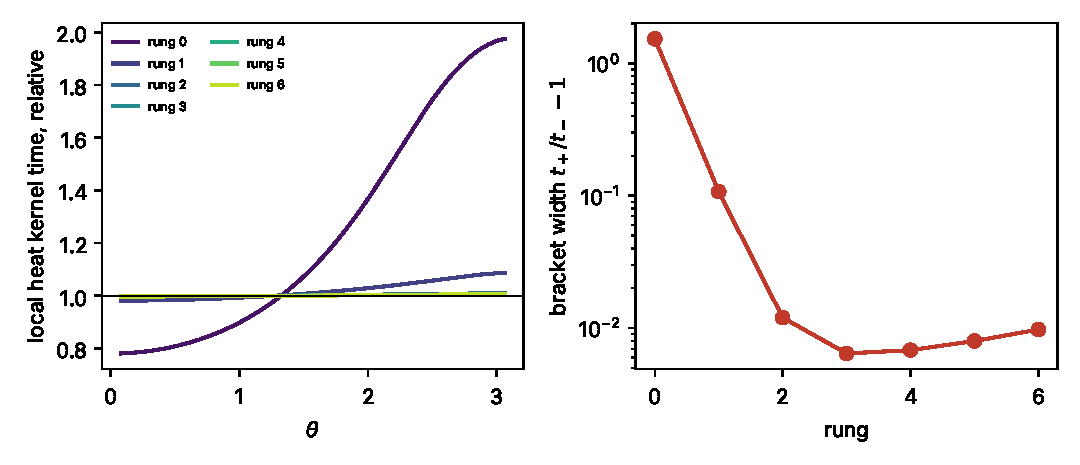
\includegraphics[width=\textwidth]{figures/local_time.pdf}
\caption[The local heat kernel time along the ladder]{Left: the local heat kernel time $t_f(\theta)$ of the plaquette law at each rung of the ladder started from the Wilson law at $\beta=2.5$, relative to the time defined by $u_2$. A heat kernel law is a horizontal line at one. Right: the width $t_+/t_--1$ of the heat kernel bracket in the likelihood ratio order.}
\label{fig:localtime}
\end{figure}

The Wilson law itself is far from the family: its local time ranges over a factor of $2.5$, short near the identity and long near the antipode, which is Proposition~\ref{prop:wilsonflow} seen pointwise. One step of the ladder cuts the width to eleven percent and a second to $1.2$ percent, after which it stays between $0.6$ and one percent. So the ladder started from the Wilson action enters a one percent neighbourhood of the heat kernel family, in the likelihood ratio order, after two rungs, and stays there through the six rungs computed. The neighbourhood does not shrink to zero: the invariant manifold of the ladder is close to the heat kernel family but is not equal to it, which is the residual error of the projection in Section~\ref{ch:verification}.

This answers the question of how to extend the monotone covering from heat kernel starts to Wilson starts: carry the pair $(t_-,t_+)$ instead of a single time. For that to be a theorem, decimation, the convolution of a law with itself, must preserve the likelihood ratio order when the law is not a heat kernel. The next section settles when it does.

\section{When does convolution preserve the likelihood ratio order?}

Let $f$ be a class function density on SU(2), and let $X$ have angle $\theta'$ and $Y$ be independent with law $f$. The angle $\psi$ of $XY$ satisfies $\cos\psi=\cos\alpha\cos\theta'-\sin\alpha\sin\theta'\cos\xi$, with $\alpha$ the angle of $Y$ and $\cos\xi$ uniform on $[-1,1]$, so the transition density from $\theta'$ to $\psi$ is
\[
q_f(\theta',\psi)=\frac{\sin\psi}{\pi\sin\theta'}\,F(\theta',\psi),\qquad F(x,y)=\int_{|x-y|}^{\min(x+y,\,2\pi-x-y)}w(\alpha)\,\mathrm d\alpha,
\]
where $w=f\sin$.
The kernel $q_f$ is totally positive of order two exactly when $F$ is.

\begin{theorem}[total positivity of convolution]\label{thm:tp2}
Let $w=f\sin$ be positive and twice differentiable on $(0,\pi)$, and put
\[
Q(\alpha)=\frac{w''(\alpha)}{w(\alpha)}=\frac{\Delta f}{f}(\alpha)-1,\qquad\Delta=\partial_\alpha^2+2\cot\alpha\,\partial_\alpha ,
\]
with $\Delta$ the radial Laplacian of the three sphere. If $Q$ is nondecreasing on $(0,\pi)$, then $F$ is totally positive of order two, and convolution with $f$ preserves the likelihood ratio order between class function laws. If $Q$ is nonincreasing, $F$ is reverse regular of order two. Equality holds throughout exactly when $w''=\lambda w$.
\end{theorem}

\begin{proof}
For $x\ge y$ with $x+y\le\pi$ put $a=x-y$, $b=x+y$ and $H=\int_a^bw$. Then $F_x=w(b)-w(a)$, $F_y=w(b)+w(a)$, $F_{xy}=w'(b)+w'(a)$, and
\[
\Psi(a,b):=F\,F_{xy}-F_xF_y=H\,\big(w'(a)+w'(b)\big)-w(b)^2+w(a)^2 .
\]
For $x+y>\pi$ the upper limit is $c=2\pi-x-y$, and the same computation gives $FF_{xy}-F_xF_y=\Psi(a,c)$. So $F$ is totally positive of order two if and only if $\Psi(a,b)\ge0$ for all $0<a<b<\pi$; $F$ is continuously differentiable across the lines $x=y$ and $x+y=\pi$ because $w$ vanishes at $0$ and $\pi$. Now
\begin{align*}
\partial_b\Psi&=w(b)\big(w'(a)-w'(b)\big)+H\,w''(b),\\
\partial_a\Psi&=w(a)\big(w'(a)-w'(b)\big)+H\,w''(a),
\end{align*}
and therefore
\[
\Big(\frac{1}{w(b)}\partial_b-\frac{1}{w(a)}\partial_a\Big)\Psi=H\,\big(Q(b)-Q(a)\big).
\]
In the coordinates $u=\int_0^bw$ and $v=\int_0^aw$ the left side is $(\partial_u-\partial_v)\Psi$. On the diagonal $u=v$, $\Psi=0$. Moving from the diagonal in the direction $(1,-1)$, which widens the interval $[a,b]$, the derivative of $\Psi$ is $(u-v)(Q(b)-Q(a))$, which is nonnegative when $Q$ is nondecreasing. Hence $\Psi\ge0$. The other cases are the same argument with the sign reversed.
\end{proof}

The equality cases are the laws with $\Delta f=(\lambda+1)f$: Haar measure and, formally, the single characters, for which the convolution kernel factorises. The condition has a second reading. Under the heat flow, $4\partial_t\log\rho=\Delta\rho/\rho$, so
\[
\partial_\alpha\,\frac{\Delta\rho}{\rho}=4\,\partial_t\partial_\alpha\log\rho .
\]
The hypothesis of Theorem~\ref{thm:tp2} is that $f$, as an initial law for the heat flow, has monotone likelihood ratio in time at time zero. Three corollaries follow at once.

\begin{corollary}\label{cor:tp2}
\begin{enumerate}
\item[(i)] Every heat kernel $K_t$ satisfies the hypothesis, by Corollary~\ref{cor:mlrall}. This is an independent proof, from the product formula, of the total positivity of order two of the radial heat semigroup on SU(2).
\item[(ii)] The Wilson law $e^{\kappa\cos\theta}$ satisfies it if and only if $\kappa\le3/2$, by Proposition~\ref{prop:wilsonflow}.
\item[(iii)] The hypothesis is preserved by the heat flow, by the maximum principle of Section~\ref{ch:proofs2} of the appendix, and the class of laws whose convolution kernels are totally positive of order two is closed under convolution, because such kernels compose.
\end{enumerate}
\end{corollary}

So if $f_1\le_{\mathrm{lr}}f_2$ and both have totally positive kernels, then $f_1^{*m}\le_{\mathrm{lr}}f_2^{*m}$ for every $m$: replace the factors one at a time. Decimation is monotone in the likelihood ratio order on that class.

One might ask whether log concavity in $\cos\theta$ is enough. It is not. Bond moved laws $K_t^k$ are log concave in $\cos\theta$ by Corollary~\ref{cor:logconc}, but
\[
\partial_\alpha\frac{\Delta(f^k)}{f^k}=k\,\partial_\alpha\frac{\Delta f}{f}+2k(k-1)\,v\,v',\qquad v=\partial_\alpha\log f,
\]
and near the antipode $v<0$ and $v'>0$, so the second term is negative and, for $k=4$, wins. A direct evaluation of $\Psi$ on a grid of pairs confirms it.

\begin{center}
\small
\begin{tabular}{lcc}
\toprule
law & share of pairs $(a,b)$ with $\Psi<0$ & where \\ \midrule
$K_2$ & 0 & \\
Wilson, $\kappa=1.4$ & 0 & \\
Wilson, $\kappa=2.5$ & 0.13 & $b$ near $\pi$ \\
$K_2^4$ & 0.06 & $b$ near $\pi$ \\
$K_1^4$ & 0.04 & $b$ near $\pi$ \\
\bottomrule
\end{tabular}
\end{center}

The violations are confined to pairs whose upper end is at the antipode, where the law has exponentially little mass at weak coupling. The conclusion, numerical for bond moved laws, is this: decimation of heat kernel laws is monotone in the likelihood ratio order; decimation of bond moved laws is monotone wherever total positivity holds, and total positivity fails only at the antipode. In the language of the renormalization group that is the large field region, which Ba\l aban's small field analysis~\cite{Ba87} leaves to a separate treatment. The comparison of Section~\ref{ch:isthere} should therefore be posed in the likelihood ratio order on a ball around the identity, together with a bound on the mass outside it.

\section{The bad cap at the antipode}

The failure can be located exactly. For $f=K_t^k$, the product formula gives, with $c=\cos\alpha$, $S_1=\sum_m(\gamma_m+c)^{-1}$ and $S_2=\sum_m(\gamma_m+c)^{-2}$,
\[
\partial_\alpha\frac{\Delta(K_t^k)}{K_t^k}=k\sin\alpha\,\Big[4\sum_m\frac{\gamma_m'(t)}{(\gamma_m+c)^2}+2(k-1)\,S_1\big(c\,S_1+(1-c^2)S_2\big)\Big].
\]

\begin{theorem}[the near hemisphere]\label{thm:hemisphere}
For every $t>0$ and every $k\ge1$ the bond moved law $K_t^k$ satisfies the hypothesis of Theorem~\ref{thm:tp2} on $(0,\pi/2]$. Consequently $\Psi(a,b)\ge0$ whenever $b\le\pi/2$, and the kernel of convolution with $K_t^k$ is totally positive of order two on the set of pairs of angles with $\theta'+\psi\le\pi/2$.
\end{theorem}

\begin{proof}
For $c\ge0$ every term in the bracket is nonnegative, since $\gamma_m>1$, $\gamma_m'>0$ and $S_1,S_2>0$. The argument of Theorem~\ref{thm:tp2} uses the monotonicity of $Q$ only on the interval $[a,b]$.
\end{proof}

Beyond the hemisphere the bracket stays positive until an angle $\alpha_*(t,k)=\pi-\eta(t,k)$. From the leading image, $v\approx-2\alpha/t$ and $v'\approx\sin^{-2}\alpha-\alpha^{-2}-2/t$, and the bracket changes sign where $\sin^{-2}\alpha-\alpha^{-2}=2k/((k-1)t)$, so
\[
\eta(t,k)\approx\sqrt{\frac{(k-1)\,t}{2k}}\qquad(t\to0).
\]
We computed $\eta$ from the image sum, and the mass that the bond moved law gives to the cap of radius $\eta$ at the antipode (Figure~\ref{fig:antipode}).

\begin{center}
\small
\begin{tabular}{ccccc}
\toprule
 & \multicolumn{2}{c}{$k=4$, four dimensions} & \multicolumn{2}{c}{$k=2$, three dimensions} \\
$t$ & $\eta$ (prediction) & mass of cap & $\eta$ (prediction) & mass of cap \\ \midrule
0.1 & 0.192 (0.194) & $10^{-148}$ & 0.154 (0.158) & $10^{-77}$ \\
0.2 & 0.271 (0.274) & $4.5\times10^{-69}$ & 0.214 (0.224) & $6.3\times10^{-37}$ \\
0.4 & 0.381 (0.387) & $10^{-31}$ & 0.294 (0.316) & $10^{-17}$ \\
0.8 & 0.528 (0.548) & $3\times10^{-13}$ & 0.372 (0.447) & $2\times10^{-8}$ \\
1.6 & 0.657 (0.775) & $2\times10^{-5}$ & 0.165 & $10^{-5}$ \\
\bottomrule
\end{tabular}
\end{center}

\begin{figure}[t]
\centering
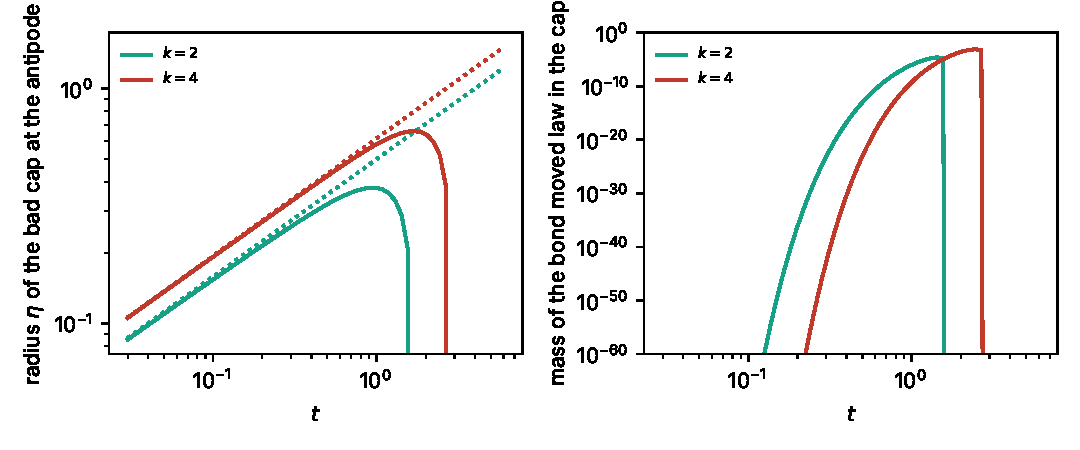
\includegraphics[width=\textwidth]{figures/antipode_radius.pdf}
\caption[The bad cap at the antipode]{Left: the radius $\eta$ of the cap at the antipode on which the bond moved law $K_t^k$ fails the total positivity condition, with the small time prediction $\sqrt{(k-1)t/(2k)}$ dotted. The cap closes at $t=2.88$ for $k=4$ and at $t=1.67$ for $k=2$. Right: the mass of the bond moved law in the cap.}
\label{fig:antipode}
\end{figure}

Three facts stand out. The small time formula is accurate to a few percent up to $t=0.8$ for $k=4$ and up to $t=0.2$ for $k=2$. The cap disappears entirely at strong coupling, according to the computed $\eta$: for $t\ge2.88$ with $k=4$, that is $\beta\le0.69$, and for $t\ge1.67$ with $k=2$, the bond moved law appears to satisfy the condition on the whole group and decimation to be monotone without qualification. This rests on the numerical $\eta$ and is not proved. And in between the cap never carries much mass: its mass is largest, $8\times10^{-4}$, at $t=2.47$ for $k=4$, and $2\times10^{-5}$ at $t=1.45$ for $k=2$. At the couplings of lattice simulations, $\beta\ge2.2$, it is below $10^{-10}$ for $k=4$.

A failure of total positivity on a set of small mass costs a small error.

\begin{proposition}[truncated monotonicity]\label{prop:truncated}
Let $q(\theta',\psi)\le M$ be a transition density that is totally positive of order two on $[0,A]\times[0,L]$, and let $f_1\le_{\mathrm{lr}}f_2$ be probability densities on $[0,\pi]$ with masses $\varepsilon_1,\varepsilon_2$ beyond $A$. Then for $\psi_1<\psi_2\le L$,
\[
(qf_2)(\psi_2)\,(qf_1)(\psi_1)-(qf_2)(\psi_1)\,(qf_1)(\psi_2)\ \ge\ -M^2\,(\varepsilon_1+\varepsilon_2+\varepsilon_1\varepsilon_2),
\]
where $(qf)(\psi)=\int f(\theta')q(\theta',\psi)\,\mathrm d\theta'$.
\end{proposition}

\begin{proof}
Split each integral at $A$. The parts over $[0,A]$ satisfy the inequality with zero on the right, by the basic composition formula, since $f_1$ and $f_2$ restricted to $[0,A]$ are still ordered and $q$ is totally positive there. Each tail is at most $M\varepsilon$ and each truncated integral at most $M$; dropping the tails from the first product and bounding them in the second gives the error term.
\end{proof}

With $A+L\le\pi/2$ the kernel of convolution with $K_t^k$ qualifies, by Theorem~\ref{thm:hemisphere}. So one step of the ladder is monotone in the likelihood ratio order on the ball of radius $L$, up to an error of at most $M^2(\varepsilon_1+\varepsilon_2+\varepsilon_1\varepsilon_2)$, with $\varepsilon_i$ the masses outside the ball of radius $A$. With $A=L=\pi/4$ the mass outside is of order $e^{-k\pi^2/(16t)}$, which is $0.05$ at $\beta=2.5$ and $4\times10^{-6}$ at $\beta=10$ for $k=4$. If the numerically determined $\eta$ is used, so that $A+L\le\pi-\eta$ and $A=L$ is just below $\pi/2$, the mass is of order $e^{-k\pi^2/(4t)}$, which is $4\times10^{-6}$ at $\beta=2.5$ and $4\times10^{-22}$ at $\beta=10$; this version is numerical. At strong coupling the cap appears, numerically, to be absent and the step monotone exactly.

\begin{quote}
\textsc{Status.} Decimation is monotone in the likelihood ratio order for heat kernel laws at every coupling; for bond moved laws on the near hemisphere, with an error that is exponentially small at weak coupling; and, numerically and not yet proved, for bond moved laws at strong coupling, $\beta\le0.69$ in four dimensions. The window $0.7<\beta<2$, together with the couplings just above $2$ where the error bound of Proposition~\ref{prop:truncated} is not yet small, and where the law is spread over the whole group and the cap has mass up to $8\times10^{-4}$, is what remains. It is the crossover, again.
\end{quote}

\section{The ladder contracts: a proof}\label{sec:contracts}\index{Hamilton, R. S.}\index{Harnack inequality}\index{maximum principle}

The inequality $R(\beta)<\beta$ of Section~\ref{ch:verification} was verified on a grid. It can be proved. The idea is to compare the bond moved law $K_t^k$ not with $K_t$ but with the heat kernel at the time flat space would give, $K_{t/k}$.

Write $x=\cos\theta$ and $G(t,x)=\partial_x\log K_t$. In flat space $\log K_t=-\theta^2/t$ and $t\,\partial_\theta\log K_t$ does not depend on $t$: the $k$th power of a Gaussian is the Gaussian at time $t/k$, and bond moving followed by decimation returns the starting time in four dimensions. On the group the same quantity moves, and it moves one way.

\begin{theorem}[time scaled likelihood ratio]\label{thm:scaledmlr}
For the SU(2) heat kernel with $u_2=e^{-3t/4}$, the function $t\,\partial_x\log K_t(x)$ is strictly decreasing in $t$ on $t>0$, for every $x\in[-1,1]$.
\end{theorem}

\begin{proof}
Three steps, with $t_1=0.1$.

\emph{Step 1, an equation.} Put $\phi=\log K_t$, $v=t\,\partial_\theta\phi$ and $z=\partial_tv$. Since $\partial_x=-(\sin\theta)^{-1}\partial_\theta$, the claim is $z>0$ on $(0,\pi)$. From $\partial_t\phi=\frac14\big(\phi''+\phi'^2+2\cot\theta\,\phi'\big)$, differentiating once in $\theta$ and once in $t$,
\[
\partial_tz=\tfrac14z''+\Big(\frac{v}{2t}+\frac{\cot\theta}{2}\Big)z'+\Big(\frac1t\Big(1+\frac{t\phi''}{2}\Big)-\frac{1}{2\sin^2\theta}\Big)z+\frac{-v}{t^2}\Big(1+\frac{t\phi''}{2}\Big).
\]
In flat space $t\phi''=-2$ and the last term, the source, vanishes.

\emph{Step 2, the source is nonnegative.} By the product formula $K_t$ is increasing in $x$, so $-v\ge0$. Hamilton's matrix Harnack inequality~\cite{Ha93} states that on a compact manifold with nonnegative sectional curvature and parallel Ricci tensor every positive solution of $\partial_\varsigma u=\Delta u$ satisfies $\nabla^2\log u+\mathbf m/(2\varsigma)\ge0$, with $\mathbf m$ the metric. The round sphere $S^3$ qualifies, our time is $\varsigma=t/4$, and the radial component of the Hessian is $\phi''$; hence $1+t\phi''/2\ge0$. So the source is nonnegative, and $z$ is a supersolution of a linear parabolic equation whose coefficient of $z$ is bounded above on $t\ge t_1$. The function $z$ vanishes at $\theta=0$ and $\theta=\pi$, where $v$ vanishes by symmetry. By the maximum principle, applied to $e^{-\lambda t}z$ with $\lambda$ larger than that bound, $z(t_1,\cdot)\ge0$ implies $z(t,\cdot)\ge0$ for all $t\ge t_1$, and the strong maximum principle makes the inequality strict on $(0,\pi)$.

\emph{Step 3, the initial layer.} It remains to show $z(t,\cdot)>0$ for $0<t\le t_1$. This is Proposition~\ref{prop:initial} below, an explicit estimate with the images of the heat kernel.
\end{proof}

\begin{figure}[t]
\centering
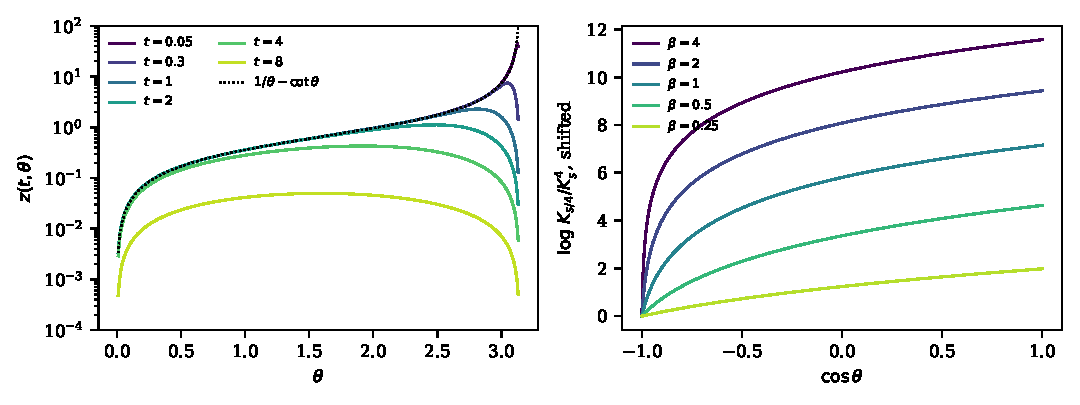
\includegraphics[width=\textwidth]{figures/contract.pdf}
\caption[The ladder contracts]{Left: $z(t,\theta)=\partial_t\big(t\,\partial_\theta\log K_t\big)$ at six times, on a logarithmic scale, with its small time limit $1/\theta-\cot\theta$; it is positive throughout, which is Theorem~\ref{thm:scaledmlr}. Right: the logarithm of the likelihood ratio $K_{t/4}/K_t^4$ against $\cos\theta$ at five couplings $\beta=2/t$, shifted to vanish at the antipode; it is increasing, which is Corollary~\ref{cor:contracts}.}
\label{fig:contract}
\end{figure}

The initial layer uses two formulas. The first is the method of images: up to a factor depending on $t$ alone,
\[
K_t\sin\theta=H(\theta,t)=\sum_{j\in\mathbb Z}\theta_j\,e^{-\theta_j^2/t},\qquad\theta_j=\theta+2\pi j,
\]
so that $z=\partial_t\big(tH'/H\big)-\cot\theta$.
The second is the product formula. The Jacobi triple product behind Theorem~\ref{thm:product} gives $K_t=\frac12\vartheta\,S_1$ with $\vartheta\propto\prod_n(1+x/C_n)$ and $S_1=\partial_x\log\vartheta=\sum_n1/(C_n+x)$. So, with $a_n=1/(C_n+x)$, $S_p=\sum a_n^p$ and $B_p=\sum C_n'a_n^p$,
\[
G=S_1-\frac{S_2}{S_1},\qquad\zeta=-\partial_t(tG)=t\Big(B_2-\frac{2B_3}{S_1}+\frac{B_2S_2}{S_1^2}\Big)-S_1+\frac{S_2}{S_1},
\]
and $z=\zeta\sin\theta$.

\begin{lemma}[perturbation]\label{lem:perturb}
Let $H=H_0(1+E)$ and let $z_0$ be defined from $H_0$ as $z$ is from $H$. If $t\le1$ and $|E|$, $|E'|$, $|\partial_tE|$, $|\partial_tE'|$ are at most $\delta\le\frac12$ at a point, then $|z-z_0|\le6\delta$ there. If moreover $|E'|$ and $|\partial_tE'|$ are at most $\theta\delta$, then $|z-z_0|\le6\theta\delta$.
\end{lemma}

\begin{proof}
$tH'/H=tH_0'/H_0+tE'/(1+E)$, and $\partial_t\big[tE'/(1+E)\big]=E'/(1+E)+t\,\partial_tE'/(1+E)-tE'\partial_tE/(1+E)^2$.
\end{proof}

\begin{proposition}[the initial layer]\label{prop:initial}
For $0<t\le0.1$ and $0<\theta<\pi$, $z(t,\theta)>0$.
\end{proposition}

\begin{proof}
Write $\epsilon=\pi-\theta$ and $u=2\pi\epsilon/t$. Three regions cover $(0,\pi)$.

\emph{Near the identity, $\theta\le\pi/2$.} Take $H_0=\theta e^{-\theta^2/t}$, for which $z_0=1/\theta-\cot\theta\ge\theta/3$. Pairing the images $j$ and $-j$,
\[
E=\sum_{j\ge1}e^{-4\pi^2j^2/t}\Big[2\cosh(\omega_j\theta)-t\omega_j^2\,\frac{\sinh(\omega_j\theta)}{\omega_j\theta}\Big],\qquad \omega_j=\frac{4\pi j}{t},
\]
an even entire function of $\theta$. Every derivative of $\sinh w/w=\int_0^1\cosh(ws)\,ds$ is bounded by $\cosh w$, so a derivative in $\theta$ costs a factor $\omega_j$ and a derivative in $t$ a factor at most $4\pi^2j^2/t^2+\omega_j\theta/t+2/t$, with an extra $\omega_j^2$ from the coefficient $t\omega_j^2$. With $\omega_j\theta\le2\pi^2j/t$ the exponentials combine to at most $e^{-2\pi^2j^2/t}$, and for $t\le0.1$ the term $j=1$ of each of $E$, $\partial_tE$, $E''$, $\partial_tE''$ is at most $1.6\times10^6\,t^{-5}e^{-2\pi^2/t}$, the remaining terms adding less than as much again. Since $t^{-5}e^{-2\pi^2/t}$ increases on $(0,0.1]$, all four are below $\delta=10^{-74}$. Because $E$ is even, $|E'|$ and $|\partial_tE'|$ are at most $\theta\delta$, and Lemma~\ref{lem:perturb} gives $z\ge\theta/3-6\theta\delta>0$.

\emph{The middle, $t/4\le\epsilon\le\pi/2$.} Take for $H_0$ the images $j=0$ and $j=-1$:
\[
H_0=2e^{-(\pi^2+\epsilon^2)/t}\big(\pi\sinh u-\epsilon\cosh u\big),\qquad\frac{tH_0'}{H_0}=2\epsilon-\frac{2\pi^2-t-2\pi\epsilon\varrho}{\mathcal D},
\]
with $\varrho=\tanh u$ and $\mathcal D=\pi\varrho-\epsilon$, and therefore
\[
z_0=z_2=\cot\epsilon+\frac1{\mathcal D}-\frac1\epsilon\Big(\frac{u}{\sinh u}\Big)^2\Big(\frac{\pi\varrho}{\mathcal D}\Big)^2\Big(1-\frac{2\epsilon^2+t}{2\pi^2}\Big).
\]
Here $u\ge\pi/2$, so $\varrho\ge0.917$, $\mathcal D\ge1.31$ and $(u/\sinh u)^2\le0.466$. The last term is at most $\epsilon^{-1}(u/\sinh u)^2(\pi\varrho/\mathcal D)^2$, which at fixed $\epsilon$ decreases as $t$ decreases, because $u$ grows; so it is enough to bound it at $t=0.1$, where $u=20\pi\epsilon$. For $\epsilon\le0.05$: $(\pi\varrho/\mathcal D)^2\le1.036$ and, with $\cot\epsilon\ge1/\epsilon-\epsilon/2$, $z_2\ge0.517/\epsilon-\epsilon/2\ge10$. For $0.05\le\epsilon\le0.1$: $u\ge\pi$, $(u/\sinh u)^2\le0.074$, $(\pi\varrho/\mathcal D)^2\le1.07$, and $z_2\ge0.92/\epsilon-0.05\ge9$. For $\epsilon\ge0.1$: $u\ge2\pi$, $(u/\sinh u)^2\le6\times10^{-4}$, $(\pi\varrho/\mathcal D)^2\le4.84$, the last term is below $0.03$, and $z_2\ge\cot\epsilon+1/\mathcal D-0.03\ge1/\pi-0.03>0.28$.

For the error, $H_0\ge1.31\,e^{-\theta^2/t}\ge1.31\,e^{-\pi^2/t}$, while the remaining images are at distance at least $5\pi/2$ from the origin, so they and their first derivatives in $\theta$ and $t$ are at most $1.6\times10^4\,t^{-3}e^{-25\pi^2/(4t)}$. From the formulas above, $|H_0'/H_0|\le19/t$, $|\partial_tH_0/H_0|\le49/t^2$ and $|\partial_t(H_0'/H_0)|\le360/t^3$. Hence $E$, $E'$, $\partial_tE$ and $\partial_tE'$ are at most $1.6\times10^7\,t^{-6}e^{-51.8/t}<10^{-200}$ for $t\le0.1$, and Lemma~\ref{lem:perturb} gives $z\ge0.28-10^{-199}>0$.

\emph{The cap, $\epsilon\le t/4$.} Here no asymptotics are needed, and the argument holds for every $t>0$. By Euler's relation for the homogeneous function $G$ of the $a_j$, $\zeta=\sum_jw_ja_j\big(tC_j'a_j-1\big)$ with $w_j=(1-p_j)^2+\sum_{n\ne j}p_n^2\ge0$ and $p_n=a_n/S_1$. With $y_j=(2j-1)t/4$, $tC_j'a_j=y_j\sinh y_j/(\cosh y_j+x)$, which is at least one when $x\le \ell(y_j)=y_j\sinh y_j-\cosh y_j$. The function $\ell$ is increasing and $\ell(y)\ge-1+y^2/2$, while $x=-\cos\epsilon\le-1+\epsilon^2/2$. So for $\epsilon\le t/4=y_1$ every term is nonnegative and those with $j\ge2$ are positive.
\end{proof}

\paragraph{\normalfont\scshape Checks.} The proof uses no computation, but each part was checked by one (\texttt{initial\_layer.py} and \texttt{ladder\_certificate.py}). The model $z_2$ agrees with $z$ computed from thirteen images in sixty digit arithmetic to the precision of the numerical derivative, and its minimum on $[t/4,\pi/2]$ is $2/\pi$, at $\epsilon=\pi/2$, for $t=0.1$, $0.03$ and $0.002$; the three lower bounds of the proof hold on a grid of four hundred points at each. Independently of the proposition, positivity of $\zeta(t_0,\cdot)$ on $[-1,1]$ was checked by an enclosure at $t_0=2$, $0.5$, $0.1$, $0.02$, $0.005$ and $0.002$: each of the four sums in $\zeta$ has positive terms decreasing in $x$, so on a box it lies between its values at the endpoints, and bisection until the lower bound is positive covers the interval with $50$ to $7370$ boxes, with an allowance of $10^{-9}$ for rounding and tails and with the sums evaluated in the variable $1+x$ to avoid cancellation at the antipode.

\begin{corollary}[the ladder contracts]\label{cor:contracts}
Let $k>1$ and $t>0$. Then $K_{t/k}/K_t^k$ is strictly increasing in $\cos\theta$: the bond moved law is strictly above the heat kernel at time $t/k$ in the likelihood ratio order of the angle used in Proposition~\ref{prop:localtime}. Consequently
\[
\frac{\int\cos\theta\,K_t^k}{\int K_t^k}<e^{-3t/(4k)},
\]
and the heat kernel projected Migdal Kadanoff map with scale factor $b$ in dimension $d$, where $k=b^{d-2}$, sends the time $t$ to $t'>b^{4-d}t$. In four dimensions $R(\beta)<\beta$ for every $\beta>0$ and every $b$. In three dimensions $t'>bt$.
\end{corollary}

\begin{proof}
$\partial_x\big[\log K_{t/k}-k\log K_t\big]=G(t/k,x)-kG(t,x)=\frac kt\big[(t/k)G(t/k,x)-tG(t,x)\big]>0$ by the theorem, since $t/k<t$. Likelihood ratio order implies the order of the means of $\cos\theta$, and the mean under $K_{t/k}$ is $u_2(t/k)=e^{-3t/(4k)}$. Decimation raises the fundamental coefficient to the power $b^2$, so $u_2'<e^{-3b^2t/(4k)}$ and $t'=-\frac43\log u_2'>b^2t/k$.
\end{proof}

Four remarks.

First, this settles the first problem of Chapter~\ref{ch:programme}: the projected ladder of SU(2) moves every coupling strictly toward strong coupling at every rung, for every scale factor. Nothing in four dimensions changes; this is a theorem about the heat kernel projection of the hierarchical model. For the exact ladder the bond moving half is the same statement, and the decimation half needs convolution to preserve the order, which is the problem of the bad cap above.

Second, the proof rests on two supports: a theorem from geometric analysis, Hamilton's inequality, used through the maximum principle; and an explicit small time estimate from the method of images, with margins of seventy orders of magnitude and more. It is not computer assisted. An enclosure at fixed time slices serves as an independent check, described above.

Third, the proof explains the direction of the flow. The decrement of the ladder is the amount by which $t\,\partial_x\log K_t$ falls between $t/k$ and $t$, and it is positive because of Hamilton's inequality, which is a statement of nonnegative curvature. In flat space there is equality and no running; on a group there is curvature and the coupling runs to strong coupling. Hamilton's inequality holds on every compact Lie group with its biinvariant metric, so the Hamilton part of Step 2 is available for SU(N), although the sign of $-v$ came from the SU(2) product formula; Steps 1 and 3 used one angle and need the Weyl chamber in general.

Fourth, the theorem has a short proof of the likelihood ratio property as a byproduct. $G=2\sum_{m<n}a_ma_n/\sum_na_n$ has $\partial G/\partial a_j=(1-p_j)^2+\sum_{n\ne j}p_n^2\ge0$ with $p_n=a_n/S_1$, and each $a_j$ decreases in $t$; so $G$ decreases in $t$, which is Corollary~\ref{cor:mlrall}.

\section{The string tension on the hierarchical lattice exists}

\begin{proposition}\label{prop:sigmaexists}
Let $u^{(m)}_2$ be the second character coefficient after $m$ steps of the ladder with bond moving power $k$ and decimation power $b^2$. If $u_2^{(m)}\to0$ and $0\le u_n^{(m)}\le(u_2^{(m)})^{n-1}$ for every $n\ge2$ and every $m$, then
\[
\sigma a^2=\lim_{m\to\infty}b^{-2m}\big(-\log u_2^{(m)}\big)
\]
exists, the convergence is geometric, and the limit is positive.
\end{proposition}

\begin{proof}
Write $v_m=-\log u_2^{(m)}$. When $u_2$ is small all higher coefficients are smaller, the law is $1+2u_2\chi_2+\cdots$ times Haar measure, and bond moving gives a second coefficient $k\,u_2(1+O(u_2))$. Decimation raises it to the power $b^2$. Hence $v_{m+1}=b^2\big(v_m-\log k+O(e^{-v_m})\big)$, and
\[
b^{-2(m+1)}v_{m+1}-b^{-2m}v_m=b^{-2m}\big(-\log k+O(e^{-v_m})\big).
\]
The increments are bounded by a geometric series, so the limit exists. Summing them from a rung $m_0$ onward, the limit is at least $b^{-2m_0}\big(v_{m_0}-\frac{b^2}{b^2-1}\log k-\varepsilon\big)$, with $\varepsilon>0$ the accumulated $O(e^{-v_m})$ terms, which can be made as small as we like by taking $m_0$ large, and which is positive as soon as $v_{m_0}$ exceeds $\frac{b^2}{b^2-1}\log k$; and $v_m\to\infty$ by hypothesis.
\end{proof}

For $b=2$ in four dimensions the threshold is $u_2<4^{-4/3}=0.157$. The hypothesis $u_2^{(m)}\to0$ is the statement that the flow reaches strong coupling, which for the projected ladder follows from Corollary~\ref{cor:contracts} and the continuity of $R$, and for the exact ladder is checked only numerically. The proposition makes precise the sense in which the ladder confines: once the flow enters the strong coupling region the string tension is fixed, up to the factor $b^{-2m}$ that counts how many rungs it took to get there. Asymptotic freedom is then the statement that the number of rungs grows linearly in $\beta$, with slope given by Theorem~\ref{thm:expansion}.

\section{The absolute string tension from the ladder}

By Proposition~\ref{prop:sigmaexists} the ladder predicts the string tension in lattice units, with no fitted constant. Under one step lengths scale by $b$ and areas by $b^2$, so
\[
\sigma a^2(\beta)=\lim_{m\to\infty}b^{-2m}\big(-\log u_2^{(m)}\big),
\]
where $u_2^{(m)}$ is the second character coefficient after $m$ steps from the Wilson law at $\beta$; the limit is reached geometrically once the flow is at strong coupling. We computed it for SU(2) in four and three dimensions (Figure~\ref{fig:mksigma}).

\begin{figure}[t]
\centering
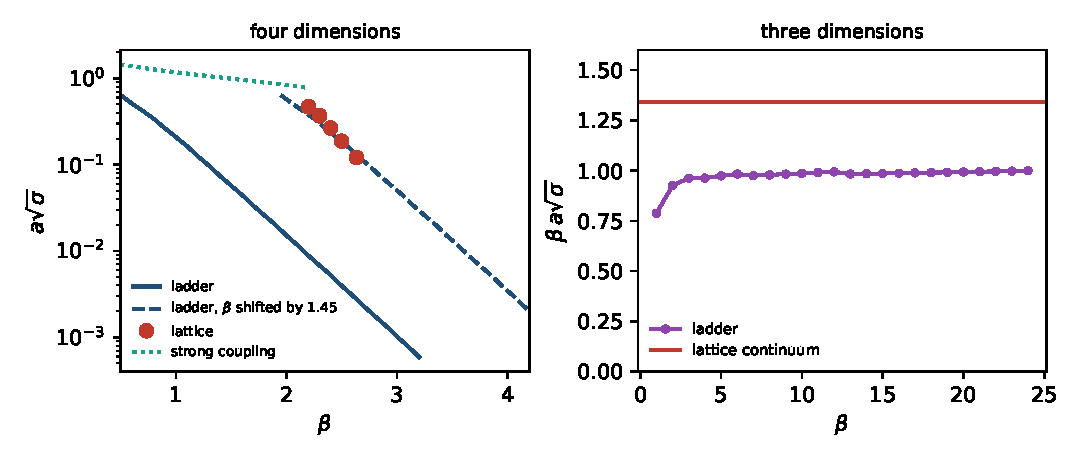
\includegraphics[width=\textwidth]{figures/mk_sigma.pdf}
\caption[Absolute string tension from the ladder]{Left: $a\sqrt\sigma$ in four dimensions from the ladder with Wilson start, the same curve shifted by $1.45$ in $\beta$, the lattice data, and the leading strong coupling formula. Right: $\beta a\sqrt\sigma$ in three dimensions from the ladder, against the continuum value $1.341$ of lattice simulations.}
\label{fig:mksigma}
\end{figure}

In four dimensions the ladder gives $a\sqrt\sigma=0.0088$, $0.0068$, $0.0053$, $0.0039$ and $0.0028$ at $\beta=2.2$, $2.3$, $2.4$, $2.5$ and $2.635$, against the lattice values $0.469$ to $0.121$: too small by a factor between $43$ and $54$ across the window. A constant factor in the lattice spacing is a shift of the coupling, here by about $1.45$: the ladder places the crossover to strong coupling near $\beta=0.8$, where the real theory has it near $\beta=2.2$. The cause is visible in the first step, where bond moving multiplies the bare coupling by $b^{d-2}=4$ before any decimation. In the language of perturbation theory the ladder has the rate of running right to ten or fifteen percent in the window and the wrong $\Lambda$ parameter by a factor of fifty.

In three dimensions the coupling has dimensions of mass and $a\sqrt\sigma$ is proportional to $1/\beta$ at weak coupling. Lattice simulations~\cite{Te99} give $\sqrt\sigma/g^2=0.3353$, that is $\beta a\sqrt\sigma=1.341$ in the continuum limit. The ladder gives values between $0.98$ and $1.00$ for $8\le\beta\le32$, with mean $0.99$, with a modulation of about two percent in $\log_2\beta$ left by the discrete scale factor. It is low by a quarter: far better than in four dimensions, because in three dimensions the scale is set by the coupling itself and not by an exponentially sensitive crossover.

\begin{quote}
\textsc{Status.} The ladder is a qualitative caricature with quantitative errors of known size: ten to fifteen percent in the rate of running, a factor of two in the two loop coefficient, a shift of $1.45$ in the four dimensional coupling, and twenty six percent in the three dimensional string tension. A comparison theorem for step 4 need not be tight, since any pair of brackets with positive decrement gives a gap. But these numbers say how far apart the brackets must be allowed to lie, and they recommend three dimensions as the place to try first; Chapter~\ref{ch:sandwich} and Section~\ref{ch:threed} take up both points.
\end{quote}

\section*{Exercises}
\begin{enumerate}
\item In Proposition~\ref{thm:mlrlarge}, prove the bound $|U_{n-1}'(x)|\le(n^3-n)/3$ on $[-1,1]$ from the identity $U_{n-1}'(1)=(n^3-n)/3$ and the fact that a Gegenbauer polynomial of positive index attains its largest modulus on $[-1,1]$ at $x=1$.
\item Show that the mixed partial of $\log(\theta e^{-\theta^2/t})$ in $t$ and $\theta$ is $2\theta/t^2$, and relate it to the small time limit of Corollary~\ref{cor:mlrall}.
\item Show that the critical points of a polynomial with real zeros are nondecreasing functions of each zero.
\item Verify Proposition~\ref{prop:wilsonflow} at $\kappa=3/2$ by expanding near $\theta=\pi$.
\item Derive the two loop decrement $\delta_{\mathrm{pert}}$ from the two loop beta function and show that its $1/\beta$ coefficient is invariant under $\beta\mapsto\beta+c$.
\item Repeat the scaling test of this chapter for SU(3) with $b=2$, using Theorem~\ref{thm:expansionN}, where the ladder predicts $d\log a/d\beta=-\log2\cdot16/9$ in units where $\beta=6/g^2$.
\end{enumerate}
